% Copyright 2008 by Mark Wibrow
%
% This file may be distributed and/or modified
%
% 1. under the LaTeX Project Public License and/or
% 2. under the GNU Public License.
%
% See the file doc/generic/pgf/licenses/LICENSE for more details.


\section{Lindenmayer System Drawing Library}

\subsection{Overview}

Lindenmayer systems (also commonly known as ``L-systems''), were originally
developed by Aristid Lindenmayer as a theory of algae growth patterns and then
subsequently used to model branching patterns in plants and produce fractal
patterns. Typically, an L-system consists of a set of symbols, each of which is
associated with some graphical action (such as ``turn left'' or ``move
forward'') and a set of rules (``production'' or ``rewrite'' rules). Given a
string of symbols, the rewrite rules are applied several times and the when
resulting string is processed the action associated with each symbol is
executed.
%
\begin{codeexample}[setup code,hidden]
    \usetikzlibrary{lindenmayersystems}
\end{codeexample}

In \pgfname, L-systems can be used to create simple 2-dimensional fractal
patterns\ldots
%
\begin{codeexample}[pre={\expandafter\let\csname pgf@lsystem@Koch curve\endcsname=\relax}]
\begin{tikzpicture}
\pgfdeclarelindenmayersystem{Koch curve}{
  \rule{F -> F-F++F-F}
}

\shadedraw [top color=white, bottom color=blue!50, draw=blue!50!black]
  [l-system={Koch curve, step=2pt, angle=60, axiom=F++F++F, order=3}]
  lindenmayer system -- cycle;
\end{tikzpicture}
\end{codeexample}
%
\noindent\ldots and ``plant like'' patterns\ldots
%
\begin{codeexample}[]
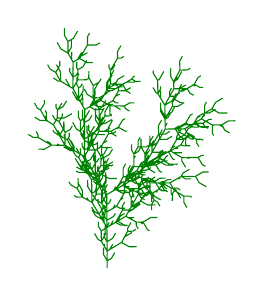
\begin{tikzpicture}
\draw [green!50!black, rotate=90]
  [l-system={rule set={F -> FF-[-F+F]+[+F-F]}, axiom=F, order=4, step=2pt,
   randomize step percent=25, angle=30, randomize angle percent=5}]
  lindenmayer system;
\end{tikzpicture}
\end{codeexample}
%
\noindent \ldots but it is important to bear in mind that even moderately
complex L-systems can exceed the available memory of \TeX, and can be very
slow. If possible, you are advised to increase the main memory and save stack
to their maximum possible values for your particular \TeX{} distribution.
However, even by doing this you may find you still run out of memory quite
quickly.

For an excellent introduction to L-systems (containing some ``really cool''
pictures -- many of which are sadly not possible in \pgfname) see \emph{The
Algorithmic Beauty of Plants} by Przemyslaw Prusinkiewicz and Aristid
Lindenmayer (which is freely available via the internet).

\begin{pgflibrary}{lindenmayersystems}
    This \pgfname-library provides basic commands for defining and using simple
    L-systems. The \tikzname-library provides, furthermore, a front end for
    using L-systems in \tikzname.
\end{pgflibrary}


\subsubsection{Declaring L-systems}

Before an L-system can be used, it must be declared using the following
command:

\begin{command}{\pgfdeclarelindenmayersystem\marg{name}\marg{specification}}
    This command declares a Lindenmayer system called \meta{name}. The
    \meta{specification} argument contains a description of the L-system's
    symbols and rules. Two commands |\symbol| and |\rule| are only defined when
    the \meta{specification} argument is executed.

    \begin{command}{\symbol\marg{name}\marg{code}}
        This defines a symbol called \meta{name} for a specific L-system,
        and associates it with \meta{code}.

        A symbol should consist of a single alpha-numeric character (i.e.,
        |A|-|Z|, |a|-|z| or |0|-|9|). The symbols |F|, |f|, |+|, |-|, |[| and
        |]| are available by default so do not need to be defined for each
        L-system. However, if you are feeling adventurous, they can be
        redefined for specific L-systems if required. The L-system treats the
        default symbols as follows (the commands they execute are described
        below):
        %
        \begin{itemize}
            \item |F| move forward a certain distance, drawing a line. Uses
                |\pgflsystemdrawforward|.
            \item |f| move forward a certain distance, without drawing a line.
                Uses |\pgflsystemmoveforward|.
            \item |+| turn left by some angle. Uses |\pgflsystemturnleft|.
            \item |-| turn right by some angle. Uses |\pgflsystemturnright|.
            \item |[| save the current state (i.e., the position and
                direction). Uses |\pgflsystemsavestate|.
            \item |]| restore the last saved state. Uses
                |\pgflsystemrestorestate|.
        \end{itemize}

        The symbols |[| and |]| act like a stack: |[| pushes the state of the
        L-system on to the stack, and |]| pops a state off the stack.

        When \meta{code} is executed, the transformation matrix is set up so
        that the origin is at the current position and the positive x-axis
        ``points forward'', so |\pgfpathlineto{\pgfpoint{1cm}{0cm}}| draws a
        line 1cm forward.

        The following keys can alter the production of an L-system. However,
        they do not store values in themselves.

        \begin{key}{/pgf/lindenmayer system/step=\meta{length} (initially 5pt)}
            How far the L-system moves forward if required. This key sets the
            \TeX{} dimension |\pgflsystemstep|.
        \end{key}

        \begin{key}{/pgf/lindenmayer system/randomize step percent=\meta{percentage} (initially 0)}
            If the step is to be randomized, this key specifies by how much.
            The value is stored in the \TeX{} macro
            |\pgflsystemrandomizesteppercent|.
        \end{key}

        \begin{key}{/pgf/lindenmayer system/left angle=\meta{angle} (initially 90)}
            This key sets the angle through which the L-system turns when it
            turns left. The value is stored in the \TeX{} macro
            |\pgflsystemrleftangle|.
        \end{key}

        \begin{key}{/pgf/lindenmayer system/right angle=\meta{angle} (initially 90)}
            This key sets the angle through which the L-system turns when it
            turns right. The value is stored in the \TeX{} macro
            |\pgflsystemrrightangle|.
        \end{key}

        \begin{key}{/pgf/lindenmayer system/randomize angle percent=\meta{percentage} (initially 0)}
            If the angles are to be randomized, this key specifies by how much.
            The value is stored in the \TeX{} macro
            |\pgflsystemrandomizeanglepercent|.
        \end{key}

        For speed and convenience, when the code for a symbol is executed, the
        following commands are available.

        \begin{command}{\pgflsystemcurrentstep}
            The current ``step'' of the L-system (i.e., how far the system
            will move forward if required). This is initially set to the
            value in the \TeX-dimensions |\pgflsystemstep|, but the actual
            value may be changed if |\pgflsystemrandomizestep| is used
            (see below).
        \end{command}

        \begin{command}{\pgflsystemcurrentleftangle}
            The angle the L-system will turn when it turns left.
            The value stored in this macro may be changed if
            |\pgflsystemrandomizeleftangle| is used.
        \end{command}

        \begin{command}{\pgflsystemcurrentrightangle}
            The angle the L-system will turn when it turns right.
            The value stored in this macro may be changed if
            |\pgflsystemrandomizerightangle| is used.
        \end{command}

        The following commands may be useful if you wish to define your own
        symbols.

        \begin{command}{\pgflsystemrandomizestep}
            Randomizes the value in |\pgflsystemcurrentstep| according to the
            current value of the key |randomize step percent|.
        \end{command}

        \begin{command}{\pgflsystemrandomizeleftangle}
            Randomizes the value in |\pgflsystemcurrentleftangle| according to
            the value of the |randomize angle percent| key.
        \end{command}

        \begin{command}{\pgflsystemrandomizerightangle}
            Randomizes the value in |\pgflsystemcurrentrightangle| according
            to the value of the |randomize angle| key.
        \end{command}

        \begin{command}{\pgflsystemdrawforward}
            Move forward in the current direction, by |\pgflsystemcurrentstep|,
            drawing a line in the process. This macro calls
            |\pgflsystemrandomizestep|. Internally, \pgfname{} simply shifts
            the transformation matrix in the positive direction of the current
            (transformed) x-axis by |\pgflsystemstep| and then executes a
            line-to to the (newly transformed) origin.
        \end{command}

        \begin{command}{\pgflsystemmoveforward}
            Move forward in the current direction, by |\pgflsystemcurrentstep|,
            without drawing a line. This macro calls
            |\pgflsystemrandomizestep|. \pgfname{} executes a transformation as
            above, but executes a move-to to the (newly transformed) origin.
        \end{command}

        \begin{command}{\pgflsystemturnleft}
            Turn left by |\pgflsystemcurrentleftangle|. Internally, \pgfname{}
            simply rotates the transformation matrix. This macro calls
            |\pgflsystemrandomizeleftangle|.
        \end{command}

        \begin{command}{\pgflsystemturnright}
            Turn right by |\pgflsystemcurrentrightangle|. Internally,
            \pgfname{} simply rotates the transformation matrix. This macro
            calls |\pgflsystemrandomizerightangle|.
        \end{command}

        \begin{command}{\pgflsystemsavestate}
            Save the current position and orientation. Internally, \pgfname{}
            simply starts a new \TeX-group.
        \end{command}

        \begin{command}{\pgflsystemrestorestate}
            Restore the last saved position and orientation. Internally,
            \pgfname{} closes a \TeX-group, restoring the transformation matrix
            of the outer scope, and a move-to command is executed to the
            (transformed) origin.
        \end{command}
    \end{command}

    \begin{command}{\rule{\ttfamily\char`\{}\meta{head}{\ttfamily->}\meta{body}{\ttfamily\char`\}}}
        Declare a rule. \meta{head} should consist of a single symbol, which
        need not have been declared using |\symbol| or exist as a default
        symbol (in fact, the more interesting L-systems depend on using symbols
        with no corresponding code, to control the ``growth'' of the system).
        \meta{body} consists of a string of symbols, which again need not
        necessarily have any code associated with them.
    \end{command}

    As an example, the following shows an L-system that uses some of these
    commands. This example illustrates the point that some symbols, in this
    case |A| and |B|, do not have to have code associated with them. They
    simply control the growth of the system.
    %
\begin{codeexample}[pre={\nullfont\expandafter\let\csname pgf@lsystem@Hilbert curve\endcsname=\relax}]
\pgfdeclarelindenmayersystem{Hilbert curve}{
  \symbol{X}{\pgflsystemdrawforward}
  \symbol{+}{\pgflsystemturnright} % Explicitly define + and - symbols.
  \symbol{-}{\pgflsystemturnleft}
  \rule{A -> +BX-AXA-XB+}
  \rule{B -> -AX+BXB+XA-}
}
\tikz\draw[lindenmayer system={Hilbert curve, axiom=A, order=4, angle=90}]
  lindenmayer system;
\end{codeexample}
    %
\end{command}


\subsection{Using Lindenmayer Systems}

\subsubsection{Using L-Systems in PGF}

The following command is used to run an L-system in \pgfname:
%
\begin{command}{\pgflindenmayersystem\marg{name}\marg{axiom}\marg{order}}
    Runs the L-system called \meta{name} using the input string \meta{axiom}
    for \meta{order} iterations. In general, prior to calling this command, the
    transformation matrix should be set appropriately for shifting and
    rotating, and a move-to to the (transformed) origin should be executed.
    This origin will be where the L-system starts. In addition, the relevant
    keys should be set appropriately.
    %
\begin{codeexample}[]
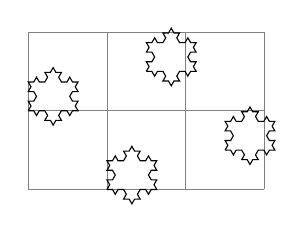
\begin{tikzpicture}
  \draw [help lines] grid (3,2);
  \pgfset{lindenmayer system/.cd, angle=60, step=2pt}
  \foreach \x/\y in {0cm/1cm, 1.5cm/1.5cm, 2.5cm/0.5cm, 1cm/0cm}{
    \pgftransformshift{\pgfqpoint{\x}{\y}}
    \pgfpathmoveto{\pgfpointorigin}
    \pgflindenmayersystem{Koch curve}{F++F++F}{2}
    \pgfusepath{stroke}
  }
\end{tikzpicture}
\end{codeexample}

    Note that it is perfectly feasible for an L-system to define special
    symbols which perform the move-to and use-path operations.
    %
\end{command}


\subsubsection{Using L-Systems in Ti\emph{k}Z}

In \tikzname, an L-system is created using a path operation. However,
\tikzname{} is more flexible regarding the positioning of the L-system and also
provides keys to create L-systems ``on-line''.

\begin{pathoperation}{lindenmayer system}{ \opt{|[|\meta{keys}|]|}}
    This will run an L-system according to the parameters specified in
    \meta{keys} (which can also contain normal \tikz{} keys such as |draw| or
    |thin|). The syntax is flexible regarding the L-system parameters and the
    following all do the same thing:
    %
\begin{codeexample}[code only]
\draw lindenmayer system [lindenmayer system={Hilbert curve, axiom=4, order=3}];
\end{codeexample}

\begin{codeexample}[code only]
\draw [lindenmayer system={Hilbert curve, axiom=4, order=3}] lindenmayer system;
\end{codeexample}

\begin{codeexample}[code only]
\tikzset{lindenmayer system={Hilbert curve, axiom=4, order=3}}
\draw lindenmayer system;
\end{codeexample}
    %
\end{pathoperation}

\begin{pathoperation}{l-system}{ \opt{|[|\meta{keys}|]|}}
    A more compact version of the |lindenmayer system| path command.
\end{pathoperation}

This library adds some additional keys for specifying L-systems. These keys
only work in \tikzname{} and all have the same path, namely, |/pgf/lindenmayer|
|system|, but the following keys are provided for convenience, so that you do
not have to keep repeating this path:

\begin{stylekey}{/pgf/lindenmayer system=\marg{keys}}
\keyalias{tikz}
    This key changes the key path to |/pgf/lindenmayer systems| and executes
    \meta{keys}.
\end{stylekey}

\begin{stylekey}{/pgf/l-system=\marg{keys}}
\keyalias{tikz}
    A more compact version of the previous key.
\end{stylekey}

\begin{key}{/pgf/lindenmayer system/name=\marg{name}}
    Sets the name for the L-system.
\end{key}

\begin{key}{/pgf/lindenmayer system/axiom=\marg{string}}
    Sets the axiom (or input string) for the L-system.
\end{key}

\begin{key}{/pgf/lindenmayer system/order=\marg{integer}}
    Sets the number of iterations the L-system will perform.
\end{key}

\begin{key}{/pgf/lindenmayer system/rule set=\marg{list}}
    This key allows an (anonymous) L-system to be declared ``on-line''. There
    is, however, a restriction that only the default symbols can be used for
    drawing (empty symbols can still be used to control the growth of the
    system). The rules in \meta{list} should be separated by commas.
    %
\begin{codeexample}[]
\tikz[rotate=65]\draw [green!60!black] l-system
  [l-system={rule set={F -> F[+F]F[-F]}, axiom=F, order=4, angle=25,step=3pt}];
\end{codeexample}
    %
\end{key}

\begin{key}{/pgf/lindenmayer system/anchor=\meta{anchor}}
    Be default, when this key is not used, the L-system will start from the
    last specified coordinate. By using this key, the L-system will be placed
    inside a special (rectangle) node which can be positioned using
    \meta{anchor}.
    %
\begin{codeexample}[]
\begin{tikzpicture}[l-system={step=1.75pt, order=5, angle=60}]
  \pgfdeclarelindenmayersystem{Sierpinski triangle}{
    \symbol{X}{\pgflsystemdrawforward}
    \symbol{Y}{\pgflsystemdrawforward}
    \rule{X -> Y-X-Y}
    \rule{Y -> X+Y+X}
  }
  \draw [help lines] grid (3,2);
  \draw [red] (0,0) l-system
    [l-system={Sierpinski triangle, axiom=+++X, anchor=south west}];
  \draw [blue] (3,2) l-system
    [l-system={Sierpinski triangle, axiom=X, anchor=north east}];
\end{tikzpicture}
\end{codeexample}
    %
\end{key}
